\documentclass[11pt,a4paper]{article}
\usepackage[T1]{fontenc}
\usepackage[utf8]{inputenc}
\usepackage{mathptmx}
\usepackage[scaled=0.9]{helvet}
\usepackage[margin=1in]{geometry}
\usepackage{setspace}
\usepackage{microtype}
\usepackage{amsmath,amssymb,amsthm}
\usepackage{graphicx}
\usepackage{booktabs,tabularx,array,multirow}
\usepackage[font=small,labelfont=bf,labelsep=period,skip=6pt]{caption}
\usepackage{enumitem}
\usepackage[round,authoryear,sort]{natbib}
\usepackage{xcolor}
\usepackage[hyphens]{url}
\usepackage[colorlinks=true,linkcolor=black,citecolor=blue!45!black,urlcolor=blue!45!black,pdftitle={Anchored to What? Price Limits, Rationed Creation and the Premiums on India's International ETFs},pdfauthor={Amish Yadav}]{hyperref}
\usepackage{titlesec}
\usepackage{placeins}
\usepackage{float}
\usepackage{fancyhdr}

\setstretch{1.22}
\setlength{\parskip}{0pt}
\setlength{\parindent}{1.4em}
\frenchspacing
\titleformat{\section}{\large\bfseries}{\thesection.}{0.5em}{}
\titleformat{\subsection}{\normalsize\bfseries}{\thesubsection}{0.5em}{}
\titlespacing*{\section}{0pt}{1.6ex plus .4ex}{0.7ex}
\titlespacing*{\subsection}{0pt}{1.2ex plus .3ex}{0.5ex}
\setlist{nosep,leftmargin=1.6em}
\renewcommand{\arraystretch}{1.12}
\newcolumntype{L}[1]{>{\raggedright\arraybackslash}p{#1}}
\newcolumntype{R}[1]{>{\raggedleft\arraybackslash}p{#1}}
\newcolumntype{Y}{>{\raggedright\arraybackslash}X}
\newtheorem{proposition}{Proposition}
\theoremstyle{definition}
\newtheorem{definition}{Definition}
\pagestyle{fancy}\fancyhf{}\renewcommand{\headrulewidth}{0pt}\fancyfoot[C]{\small\thepage}
\newcommand{\fund}[1]{\textsc{\MakeLowercase{#1}}}
\newcommand{\NAV}{\mathrm{NAV}}
\newcommand{\FV}{\mathrm{FV}}
\newcommand{\tabnote}[1]{\par\smallskip\begin{minipage}{\linewidth}\footnotesize\setstretch{1.0}#1\end{minipage}}
\newcommand{\mcReps}{240}
\newcommand{\mcShareA}{35}
\newcommand{\mcShareB}{60}
\newcommand{\mcShareC}{80}
\newcommand{\mcBiasNaiveA}{10}
\newcommand{\mcBiasNaiveC}{18}
\newcommand{\mcBiasMovMin}{$-$0.7}
\newcommand{\mcBiasMovMax}{1.3}
\newcommand{\mcBiasFixMin}{1.6}
\newcommand{\mcBiasFixMax}{3.0}
\newcommand{\mcRmseMovA}{7.6}
\newcommand{\mcRmseFixA}{9.2}
\newcommand{\mcRmseMovC}{13.9}
\newcommand{\mcRmseFixC}{13.7}
\newcommand{\mcSizeMovMin}{6}
\newcommand{\mcSizeMovMax}{15}
\newcommand{\mcBelowMovMin}{5}
\newcommand{\mcBelowMovMax}{8}
\newcommand{\mcPlugMovMin}{6}
\newcommand{\mcPlugMovMax}{18}
\newcommand{\mcPowMovLoMin}{90}
\newcommand{\mcPowMovLoMax}{95}
\newcommand{\mcPowMovHiMin}{99}
\newcommand{\mcPowMovHiMax}{99}
\newcommand{\mcSizeNaiveMin}{26}
\newcommand{\mcSizeNaiveMax}{89}
\newcommand{\mcIotaNaiveMin}{28}
\newcommand{\mcIotaNaiveMax}{47}


\begin{document}
\begin{titlepage}
\thispagestyle{empty}
\begin{center}
\vspace*{1.2cm}
{\LARGE\bfseries Anchored to What?\par}
\vspace{0.35cm}
{\Large Price Limits, Rationed Creation and the Premiums\\[0.15em] on India's International ETFs\par}
\vspace{1.0cm}
{\large Amish Yadav\footnote{Mukesh Patel School of Technology Management \& Engineering, SVKM's NMIMS, Mumbai, India. Literature search, drafting and code were assisted by an AI system (Claude, Anthropic); the author is responsible for the content. The author holds no position in the funds studied and will not trade them during the study. No funding was received.}\par}
\vspace{0.25cm}
{\normalsize Mukesh Patel School of Technology Management \& Engineering, NMIMS, Mumbai\par}
\vspace{0.5cm}
{\normalsize Second draft: 12 November 2026\par}
\vspace{0.15cm}
{\small Pre-results working paper. Design, measures and tests are fixed here; no estimate comes from the study's own panel, which is under construction.\par}
\end{center}
\vspace{0.8cm}
\begin{center}\textbf{Abstract}\end{center}
\vspace{-0.2cm}
\begin{quote}\setstretch{1.1}\small
India caps what its mutual funds may invest abroad, and since 2022 the cap has rationed the creation of units in its six listed international exchange-traded funds. Until 4 September 2026 a daily price band anchored to a lagged net asset value (NAV) capped their premiums; exchange files show that on the last day of that regime five of the six closed exactly at the ceiling. On 7 September the band was re-anchored to the previous close. One fund closed 235\% above NAV on the ninth session that followed, and on 9 November the six funds were worth Rs 4,875 crore more on the exchange than at NAV. This paper argues that when arbitrage is blocked, the reference price of a price limit decides whether mispricing is bounded: a value anchor is a fence, a price anchor only a speed limit. It sets out a design to measure how much of the later premium the old band had hidden and how much the new band induced, using a censored autoregression whose ceiling moves each day, and shows by simulation that the estimator recovers a known hidden premium, while ignoring the censoring mistakes hidden demand for induced demand. It dates quota-rationed creations from the exchange's unit counts, and it fixes tests for the planned return to a NAV anchor on 1 April 2027, a switch that cannot be smooth for any fund trading more than 20\% above NAV.
\end{quote}
\vspace{0.3cm}
\noindent{\small\textbf{Keywords:} exchange-traded funds; price limits; reference price; limits to arbitrage; capital controls; censored regression; pre-registration; India.\par}
\vspace{0.15cm}
\noindent{\small\textbf{JEL classification:} G12, G14, G18, G23, F38.\par}
\end{titlepage}
\setcounter{page}{1}

%=====================================================================
\section{Introduction}
On 18 September 2026 a unit of the Motilal Oswal Nasdaq Q50 ETF closed at Rs 396.30 on the National Stock Exchange of India (NSE). The fund's net asset value (NAV) for that date was Rs 118.14 \citep{indmoney2026unwind}. Buyers paid Rs 3.35 for each rupee of Nasdaq-listed shares the fund held. Two weeks earlier, on 4 September, the same unit had closed 19.5\% above NAV. The fifty companies in the fund did not triple in value in between. A trading rule changed.

An exchange-traded fund (ETF) normally trades near NAV because market makers can create new units at NAV when the price is higher and redeem units when it is lower \citep{bendavid2017exchange}. India caps what its mutual funds may invest abroad, at US\$7 billion for the industry and US\$1 billion for a fund house \citep{bs2021limit}, and the caps have bound since early 2022 \citep{pti2022resume}. An ETF that holds foreign shares must buy more of them to create a unit, so for India's six listed international ETFs creation has been rationed for most of the period since. Redemption still works. The funds behave like closed-end funds whose supply can shrink and can grow only when their fund house finds room under its cap.

A second rule hid the consequences. Exchanges allowed an ETF to trade only within 20\% of its NAV of two days earlier \citep{sebi2026circular}, and the premiums of these funds pressed against that ceiling. Exchange and fund-industry files for 4 September 2026, the last session under that rule, show five of the six funds closing exactly at the upper limit, to the paisa (Section~\ref{sec:evidence}). On 7 September the Securities and Exchange Board of India (SEBI) moved the band's base to the previous day's closing price \citep{sebi2026circular,sebi2026ext}. The change answered a problem in gold and silver ETFs, whose prices had outrun a stale NAV base early in 2026 \citep{sebi2026cp}. For a fund that cannot create units it removed the ceiling: each close became the next day's base, so a premium could compound by up to 20\% a day.

This paper is about that base. Research on price limits asks whether limits should exist and how wide they should be; in every case studied the limit is anchored to the previous close or settlement price, and the asset has no published value against which a limit could be set instead. India's ETFs had a limit anchored to value, then one anchored to price, in the same securities, with the barrier to arbitrage unchanged. The two anchors do different jobs. A limit anchored to value is a fence: it bounds how far price can stand from value, whatever buyers want. A limit anchored to price is a speed limit: it bounds each day's move and places no bound on where the price ends up. The fence was never designed as one. SEBI's stated concern was the staleness of the base, and neither its consultation paper nor its circular mentions funds that cannot create units.

The re-anchoring raises a question that the price path alone cannot answer. The 235\% premium may be demand that existed all along and that the fence had hidden. Or the new band may have created demand that did not exist before: a run of upper-limit closes draws attention and new buyers \citep{seasholes2007predictable}, and buyers extrapolate from the run itself \citep{barberis2018extrapolation,pearson2021chinese}. Call the first part revealed and the second induced. The distinction matters for policy. If the premium was revealed, the old band concealed a shortage that the cap on overseas investment had created, and the new band only made it visible. If it was induced, the choice of anchor itself moved prices away from value. The pre-change data can separate the two, because under the old band the premium was free on some days and capped on others, and the cap sat at a different level each day for reasons unrelated to demand.

The setting has three features that studies of mispricing rarely have together. The asset's value is published every day. The barrier to arbitrage is a written regulation whose bite can be read each day from the exchange's record of units outstanding. And the rule that bounds the price changed on one known date and is due, as a regulatory target, to change again on 1 April 2027, when the base is to become the previous day's NAV. Work on limits to arbitrage \citep{shleifer1997limits}, closed-end funds \citep{lee1991investor} and speculative bubbles \citep{xiong2011chinese} has usually had to estimate value, infer the barrier, or both.

The paper makes four contributions, and it is careful about what it does not claim.
\begin{enumerate}
\item \emph{The anchor as the treatment.} It is, to our knowledge, the first study of a change in the reference price of a daily price limit, from a lagged fundamental value to the previous close, in the same securities. Section~\ref{sec:framework} states what each anchor can and cannot bound, and shows that a return from a price anchor to a value anchor cannot be smooth: on the day of the switch the price of a fund trading 86\% above NAV must fall by at least 36\%.
\item \emph{Revealed against induced.} It sets out a method to estimate the premium that a value-anchored limit censored, and to split the premium observed afterwards into the part the rule revealed and the part it induced. The ceiling in the censored model is the exchange's official band relative to fair value, which moves each day. A Monte Carlo study shows that the estimator recovers a known hidden premium with little bias, that an analysis which ignores the censoring would report induced demand where there is none, and that the test needs its critical values calibrated when most days are capped (Section~\ref{sec:design}).
\item \emph{Rationing dated from exchange records.} It uses the exchange's daily count of units outstanding to date quota-rationed creations. The count contradicts the common account that creation in these funds has been shut since 2022 or 2024: one fund's units grew four and a half times between July 2024 and April 2026, in exact multiples of its creation unit. Each creation is a supply shock of known size.
\item \emph{A test fixed before the outcome.} It specifies tests for April 2027, with three branches and five predictions, before any 2027 observation exists (Section~\ref{sec:april}).
\end{enumerate}
The paper does not claim to be the first on suspended creation, which \citet{johnson2016essays} studies in exchange-traded notes, or on premiums behind capital controls, which the literature on closed-end country funds established \citep{bonserneal1990international}. It does not claim that buyers were irrational: daily data cannot identify who bought, and the April switch is a target that may be delayed. And six funds from three fund houses are a case, not a sample of ETFs.

This is a pre-results paper. The study's own panel is under construction, and no hypothesis is tested here. What the paper does report from primary sources is limited to exchange and fund-industry files for a handful of dates, which are enough to establish four facts: that five of six funds sat at the ceiling when the fence came down; that the fund houses' indicative NAVs for the US-linked funds move with the rupee and not with the underlying shares; that creation was rationed in exact creation units and stopped entirely from April 2026; and that on 9 November 2026 holders of the six funds owned units priced Rs 4,875 crore above the value of what the funds held. Press figures are used for the dates in between and are labelled as such. Appendix~\ref{app:protocol} records what had been seen when each element of the design was fixed.

India has seen the mirror image. In the 1990s and 2000s foreigners could buy depositary receipts of Indian companies abroad more freely than the shares themselves, and the receipts traded above the local shares \citep{jithendranathan2000barriers,stigler2010understanding}; those of Infosys averaged a premium of about 50\% in New York \citep{financeasia2003}, which \citet{puthenpurackal2006explaining} attributes to limited supply, downward-sloping demand and trend-chasing by small investors. Then foreigners overpaid in New York for an Indian share; now residents overpay in Mumbai for American ones. The control is of the same kind and its direction is reversed.

Section~\ref{sec:institutions} sets out the institutions. Section~\ref{sec:framework} gives the framework. Section~\ref{sec:literature} places the paper in the literature. Section~\ref{sec:hypotheses} states the hypotheses, Section~\ref{sec:data} the data and measures and Section~\ref{sec:design} the empirical design, with the simulation. Section~\ref{sec:evidence} reports the evidence available before the panel. Section~\ref{sec:april} fixes the tests for April 2027. Section~\ref{sec:limits} states the limitations and Section~\ref{sec:conclusion} concludes.

%=====================================================================
\section{Institutional Setting}\label{sec:institutions}
\subsection{Creation, redemption and who may use them}
An ETF publishes a NAV once a day and an indicative NAV (iNAV) during trading hours. Units are created and redeemed in blocks: 250,000 units for the Motilal Oswal Nasdaq 100 ETF \citep{motilal2026sid} and 600,000 for the Nasdaq Q50 ETF \citep{indmoney2026unwind}. Only market makers and investors dealing in Rs 25 crore or more transact directly with the fund house \citep{mirae2026factsheet}; everyone else trades on the exchange. Arbitrage therefore rests on a few market makers and on the fund house's ability to issue.

\subsection{Caps on overseas investment}
The industry limit of US\$7 billion dates from 2008 \citep{lawasia2026}. In November 2020 SEBI raised the limit per fund house to US\$600 million \citep{bs2020limit} and in June 2021 to US\$1 billion, with a separate industry pool of US\$1 billion, and US\$300 million per house, for investment in foreign-listed ETFs \citep{bs2021limit}. On 18 January 2022 Motilal Oswal suspended the issuance of units in its two Nasdaq ETFs to manage its limit \citep{bs2022motilal}, and fresh overseas subscriptions stopped across the industry from 1 February 2022. In June 2022 SEBI let funds resume, but only up to the room each fund house had on 1 February 2022 \citep{pti2022resume}. Mirae Asset stopped accepting direct creation requests in its three overseas ETFs from 5 January 2024 \citep{mirae2024addendum}, and the pool for foreign-listed ETFs filled in April 2024 \citep{zerodha2024etf}. The Reserve Bank of India has declined requests to raise the limits \citep{bs2023rbi}. Several fund houses shut overseas schemes again between April and July 2026 \citep{outlook2026menu}, and no increase had been announced by 11 November 2026.

Which limit binds the six funds is often misreported. Press accounts blame the US\$1 billion pool for foreign-listed ETFs and date the end of creation to April 2024 \citep[for example][]{vr2026up41}. That pool governs Indian funds that buy ETFs listed abroad. The six funds studied here hold foreign shares directly, so they draw on their fund house's room under the US\$7 billion limit, frozen at its level of 1 February 2022. Three facts support this reading. Motilal Oswal suspended ETF issuance in January 2022, when the pool for foreign-listed ETFs was not yet full \citep{bs2022bind}. Mirae Asset's notice of January 2024 ties its suspension to SEBI's instruction of January 2022, which concerned the US\$7 billion limit. And Mirae stopped creation three months before the pool for foreign-listed ETFs filled.

The distinction has a consequence that the design relies on. Room is counted per fund house, not per scheme, and is freed by redemptions from any of the house's overseas schemes. A fund house can therefore still create ETF units when room appears elsewhere in its range. Creation is rationed by the fund house; it is not prohibited scheme by scheme. How a fund house allocates freed room among its schemes and market makers is not disclosed.

Residents have another legal route abroad. The Liberalised Remittance Scheme allows US\$250,000 a year, with tax collected at source of 20\% on the amount above Rs 10 lakh, creditable against income tax \citep{bt2026lrs}. A premium paid only for access to foreign shares should be bounded by the cost of this route, which is far below the premiums observed.

\subsection{Three price-band regimes}
Table~\ref{tab:regimes} sets out the regimes. In each, the price $P_{i,t}$ of fund $i$ on day $t$ must satisfy
\begin{equation}\label{eq:band}
(1-b_t)\,B_{i,t}\;\le\;P_{i,t}\;\le\;(1+b_t)\,B_{i,t},
\end{equation}
where $B_{i,t}$ is the base and $b_t$ the half-width of the band.

\begin{table}[!t]
\centering\small
\caption{Price-band regimes for equity ETFs}\label{tab:regimes}
\begin{tabularx}{\textwidth}{L{2.0cm}L{2.3cm}L{3.2cm}YL{3.0cm}}
\toprule
Regime & In force & Base $B_{i,t}$ & Band & Bound on the premium\\
\midrule
NAV, lagged & To 4 Sep 2026 & Closing NAV of $t-2$ & Fixed $\pm 20\%$ & Level bounded; the bound moves with the two-day change in NAV\\
Previous close & From 7 Sep 2026 & Average price of the last 30 minutes of $t-1$; else last trade; else latest NAV & $\pm 10\%$; widened by 5\% of the base after a cooling-off of 15 minutes (5 in the last half-hour), at most twice in a direction & None on the level; at most 20\% a day\\
NAV, previous day & Target: 1 Apr 2027 & Closing NAV of $t-1$ & As above & Level bounded again; a forced jump on the first day\\
\bottomrule
\end{tabularx}
\tabnote{Sources: \citet{sebi2026circular}, paragraphs 2, 4.1, 4.2, 4.4 and 5.1; \citet{nse2026circular}. The average price is volume-weighted. The date on which the first regime began has not been established. Overnight and liquid ETFs keep a fixed 5\% band; gold and silver ETFs start at 6\% and widen in steps of 3\% without a cap.}
\end{table}

Under the first regime the base was the closing NAV of two days earlier and the band a fixed 20\%. The lag was not arbitrary. A scheme investing overseas may publish its NAV until 10 a.m.\ on the next business day \citep{sebi2023nav}, after the market has opened, so when the band for day $t$ is set the newest NAV in existence is that of $t-2$ (Figure~\ref{fig:timeline}). In the last week of January 2026 gold and silver moved faster than that base, and exchanges used a more recent one for bullion ETFs as an interim step \citep{sebi2026cp}. SEBI's consultation paper of 13 February 2026 proposed three alternatives: the previous close, the average iNAV of the last half hour, or the previous day's NAV where available. Its evidence was that more than 99.8\% of single-day moves in equity and debt ETFs between April and December 2025 stayed within 10\%. It compared prices with previous closes. It did not discuss distance from NAV, overseas ETFs or constraints on creation.

\begin{figure}[!t]
\centering
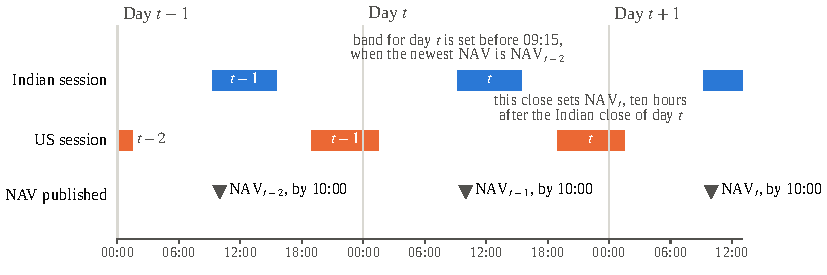
\includegraphics[width=\textwidth]{figures/fig2_timeline.pdf}
\caption{What is known when, for a US-linked fund. Times are Indian Standard Time, with US markets on summer time. The NAV dated $t$ uses the US close of date $t$, which falls ten hours after Indian trading ends, and is published by 10:00 on $t+1$. When the band for day $t$ is set, the newest NAV in existence is that of $t-2$.}\label{fig:timeline}
\end{figure}

The circular of 15 June 2026 chose the previous close, defined as the volume-weighted average price of the last 30 minutes, and recorded that the previous day's NAV was operationally difficult to use (paragraph 4.1). Equity and debt ETFs start each day with a 10\% band. When trades occur at 9.90\% from the base a cooling-off of 15 minutes follows, and the band then widens by 5\% of the base, at most twice in each direction and only on the side the price is moving (paragraph 5.1). Paragraph 4.4 directs exchanges and fund houses to resolve jointly the operational difficulties of using the previous day's closing NAV as the base, with effect from 1 April 2027. The circular does not mention overseas ETFs or the creation of units. The start was moved from 1 to 7 September at the exchanges' request \citep{sebi2026ext}, and NSE's implementing circular followed on 1 September \citep{nse2026circular}.

Whether the rule covered international ETFs was unclear to at least one large broker. On 2 September a user of its forum asked, and warned that prices could run without a NAV anchor; staff first answered that the rule did not apply, and corrected the answer on 7 September \citep{zerodha2026forum}. The risk was foreseeable and was foreseen. Both exchanges issued press releases on 25 September. NSE's states that mutual funds have fully used their overseas limits, that the creation of new units in these ETFs is restricted, and that buyers at steep premiums face an abrupt fall in price unrelated to the underlying shares, including if the limits are raised or when the base migrates to NAV under paragraph 4.4 \citep{nse2026press,bse2026press}. NSE repeated the caution on 7 October \citep{reuters2026nse}, and at least one fund house warned investors about its own ETFs \citep{cafemutual2026mirae}.

Cautions were the only instrument used. Other markets with quota-bound or issuance-bound products intervene on the premium itself. China's exchanges and fund managers publish risk warnings and halt trading in cross-border ETFs when premiums are high, usually for an hour and in January 2025 for whole days \citep{bloomberg2025halts}; one fund issued more than a hundred warnings and was halted nearly forty times in the first quarter of 2026 \citep{yicai2026quota}. Korea, after leveraged oil notes traded at several times their indicative value in April 2020 \citep{asiae2020etn}, designates products whose price strays from value beyond a threshold, moves them to single-price auctions and suspends them if the gap persists \citep{fsc2020measures}. These are triggers anchored to value. India's old band was, in effect, a rule of the same family, and the framework that replaced it has none.

\subsection{NAV timing and the indicative NAV}
A check on seven consecutive NAV dates in September 2026 found that the Nasdaq 100 ETF's NAV dated $t$ moves with the Nasdaq-100 close of US date $t$ and the exchange rate, not with the previous US session. That close comes about ten hours after Indian trading ends. The premium usually quoted, the close over the same-date NAV, therefore divides a price by a value determined later. The error is not small. On 9 November 2026 the Nasdaq Q50 ETF closed at Rs 229.67; the NAV displayed by the exchange at that close was Rs 110.89, and the NAV later published for 9 November was Rs 114.38. The quoted premium for the day is 100.8\%; against what was known at the close it was 107.1\%.

The indicative NAV does not fill the gap. Motilal Oswal states that the iNAV of its two Nasdaq ETFs is the previous day's closing NAV adjusted only for currency movement \citep{motilal2026inav}. Values saved from the fund houses' own pages after the close of 9 November agree: the iNAVs of the two Motilal Oswal funds stood 0.187\% below the previous NAV, the same to three decimal places for both, although the two funds' NAVs for that date turned out 3.2\% and 3.4\% higher. The iNAVs of Mirae Asset's two US-linked funds stood 0.08\% below their previous NAVs, again the same for both, which is what a currency-only adjustment implies; that single observation needs confirming against live sessions. Neither published number is a contemporaneous value.

The timing also bears on April 2027. A US-linked fund's NAV for $t-1$ is not due before the market opens on $t$, so a literal previous-day NAV base cannot be set before trading starts. Exchanges must use an older NAV for these funds, reset the band during the session, or delay. Any NAV anchor restores a ceiling near 20\%.

\subsection{Feeder funds}
Funds of funds that invest in these ETFs value their holdings at the exchange price \citep{vr2026fof}, so the premium sits inside the feeder's own NAV. The feeders are large holders. Rough figures from public sources put the holding of Mirae Asset's NYSE FANG+ feeder at 43\% to 50\% of that ETF's units.

Feeders were a channel of demand only while they could take new money, and they cannot. Motilal Oswal's Nasdaq 100 fund of funds stopped lump sums in January 2022, stopped registering new instalment plans in December 2024 and paused existing ones from 5 January 2025, citing exhausted overseas limits \citep{et2025motilal}. A feeder that must stop taking money for that reason was being supplied by creation, not by purchases on the exchange. Mirae Asset's feeders accept only instalment plans registered before its January 2024 suspension \citep{mirae2024addendum}. What remains is the other direction. An investor who redeems from a feeder is paid the feeder's NAV, which is struck on the ETF's exchange price, and the feeder sells ETF units on the exchange to pay. Feeder redemptions therefore put units on the market and let long-standing holders cash the premium. Two things follow for the design: float must be measured net of feeder holdings, and feeder flows are expected to be a source of supply when premiums are high.

%=====================================================================
\section{A Fence and a Speed Limit}\label{sec:framework}
This section states what a price limit can bound when creation is rationed, as a function of what the limit is anchored to. The results are arithmetic, but they organise the rest of the paper.

Let $V_{i,t}$ be the value of a unit of fund $i$ at the close of day $t$ and $P_{i,t}$ its closing price. The premium is $\pi_{i,t}=\ln(P_{i,t}/V_{i,t})$. With creation rationed, the supply of units is fixed from day to day and price is set by demand. Let $P^{*}_{i,t}$ be the price that would clear the market on day $t$ if no price limit applied, and $\pi^{*}_{i,t}=\ln(P^{*}_{i,t}/V_{i,t})$ the \emph{latent premium}. A daily limit of half-width $b$ around a base $B_{i,t}$ restricts price as in~\eqref{eq:band}.

\begin{definition}
The limit has a \emph{value anchor} with lag $\ell\ge 1$ if $B_{i,t}=V_{i,t-\ell}$. It has a \emph{price anchor} if $B_{i,t}=P_{i,t-1}$.
\end{definition}

\begin{proposition}[Fence]\label{prop:fence}
Under a value anchor with lag $\ell$,
\begin{equation}\label{eq:fence}
\pi_{i,t}\;\le\;c_{i,t}\;\equiv\;\ln(1+b)-\ln\!\left(\frac{V_{i,t}}{V_{i,t-\ell}}\right)\qquad\text{for every } t,
\end{equation}
whatever the latent premium. The observed premium is $\pi_{i,t}=\min(\pi^{*}_{i,t},\,c_{i,t})$ whenever $\pi^{*}_{i,t}$ lies above the lower limit.
\end{proposition}

The bound in~\eqref{eq:fence} does not depend on demand or on past prices. It does depend on how value has moved over the lag. With $b=0.2$ and $\ell=2$, the ceiling on the premium is 16.5\% after a two-day rise in value of 3\% and 23.7\% after a fall of 3\%. This is why premiums under the old band were reported between 19\% and 24\%, and it is what makes the premium a censored observation of demand with a censoring point that changes daily for reasons unrelated to demand.

\begin{proposition}[Speed limit]\label{prop:speed}
Under a price anchor, for any $k\ge 1$,
\begin{equation}\label{eq:speed}
\pi_{i,t}-\pi_{i,t-k}\;\le\;k\ln(1+b)-\ln\!\left(\frac{V_{i,t}}{V_{i,t-k}}\right),
\end{equation}
and there is no bound on $\pi_{i,t}$. With value constant, a latent premium $\pi^{*}$ is reached from $\pi_{0}$ in at most $\lceil(\pi^{*}-\pi_{0})/\ln(1+b)\rceil$ sessions.
\end{proposition}

A price anchor bounds the day's return, which is what a control on volatility is for. It says nothing about the distance between price and value, because the base inherits whatever distance already exists. The Nasdaq Q50 ETF needed at least six sessions of 20\% rises to go from its close of Rs 141.93 on 4 September to Rs 396.30; it took nine.

\begin{proposition}[Cliff]\label{prop:cliff}
Let the anchor change from price to value on day $T$, and let $\Pi=P_{i,T-1}/V_{i,T-\ell}-1$ be the premium of the last close over the anchoring value. If $\Pi>b$, the price on day $T$ must fall by at least
\begin{equation}\label{eq:cliff}
1-\frac{1+b}{1+\Pi}
\end{equation}
from the previous close. Before $T$ a falling price can lose at most $b$ a day, so bringing the premium inside the new band in advance takes at least $\lceil \ln\!\big((1+\Pi)/(1+b)\big)/\ln\!\big(1/(1-b)\big)\rceil$ sessions of lower-limit closes.
\end{proposition}

The return to a value anchor is therefore discontinuous for any fund whose premium exceeds the band. At a premium of 86\%, the level of the Nasdaq Q50 ETF on 4 November, the forced fall is 36\%; under the present design, in which the band starts the day at 10\%, the first trade must be at least 41\% below the previous close. Figure~\ref{fig:cliff} plots~\eqref{eq:cliff}. A holder who expects the switch has two ways out: sell before $T$ at a price that others are still willing to pay, or bear the jump. Section~\ref{sec:april} turns this into predictions.

\begin{figure}[!t]
\centering
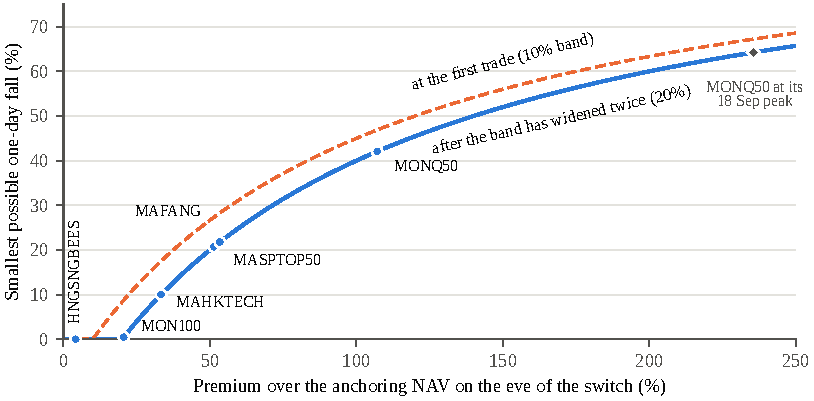
\includegraphics[width=0.92\textwidth]{figures/fig5_cliff.pdf}
\caption{The cliff. The smallest one-day fall forced on a fund when the band is re-anchored from the previous close to NAV, as a function of its premium on the eve of the switch (Proposition~\ref{prop:cliff}). Circles place the six funds at their premiums over the last known NAV on 9 November 2026 (Table~\ref{tab:cross}).}\label{fig:cliff}
\end{figure}

\paragraph{Revealed and induced.} Let $T_0$ be the last day of the value anchor. Write the latent premium after the change as the path it would have followed under the law of motion that governed it before the change, plus a remainder:
\begin{equation}\label{eq:split}
\pi_{i,t}\;=\;\underbrace{\mathrm{E}\big[\pi^{*}_{i,t}\,\big|\,\mathcal{F}_{T_0}\big]}_{\text{revealed}}\;+\;\underbrace{\pi_{i,t}-\mathrm{E}\big[\pi^{*}_{i,t}\,\big|\,\mathcal{F}_{T_0}\big]}_{\text{induced, plus news}},\qquad t>T_0,
\end{equation}
where $\mathcal{F}_{T_0}$ is the information in prices, ceilings and covariates up to $T_0$. The first term is demand that the fence was hiding. The second is zero on average if the change of anchor did nothing but remove the fence. It is positive if the price-anchored band added demand, as a run of upper-limit days would if it drew attention or was extrapolated. Figure~\ref{fig:fence} illustrates both cases with a simulated path. Section~\ref{sec:design} estimates the first term from pre-change data with a censored autoregression and reads the second as the residual.

\begin{figure}[!t]
\centering
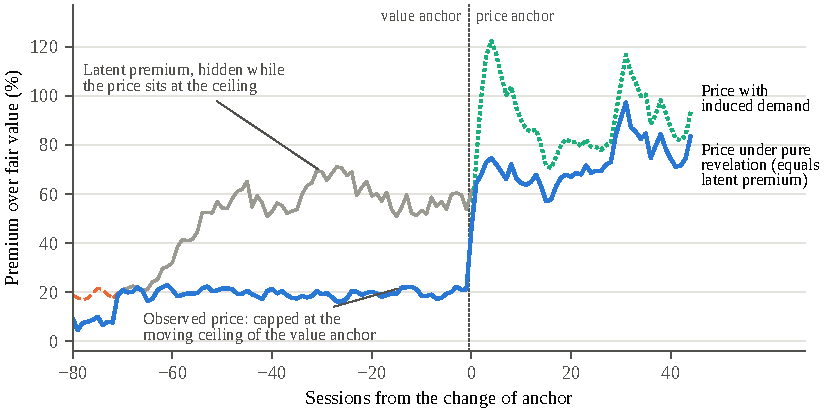
\includegraphics[width=0.92\textwidth]{figures/fig3_fence_speed.pdf}
\caption{A fence and a speed limit: simulated illustration. The grey line is a latent premium that follows a first-order autoregression. Before session 0 the price (solid) is the lower of the latent premium and a ceiling that moves with the two-day change in value (dashed). From session 0 the band is anchored to the previous close: the price may move 20\% a day and reaches the latent premium within a few sessions. The dotted line adds buying that responds to the previous day's rise and then decays. The data are simulated and are not estimates for any fund.}\label{fig:fence}
\end{figure}

Nothing here says that a value anchor is the better rule. A fence binds when value itself moves faster than a stale base, which is the problem SEBI set out to fix in bullion ETFs, and it prevents the price from showing a shortage that is real. The claim is narrower: the two anchors bound different things, and where arbitrage is blocked the difference is the difference between a premium of 20\% and one of 235\%.

%=====================================================================
\section{Related Literature}\label{sec:literature}
\paragraph{ETF pricing and suspended creation.} ETF prices deviate from NAV most in funds that hold international or illiquid assets \citep{petajisto2017inefficiencies,engle2006premiums}, in part because NAV is stale when the home market is closed \citep{levy2013overreaction}. The deviation has been split into price discovery and transitory noise \citep{madhavan2016price}, and creation flows have been shown to reveal non-fundamental demand \citep{brown2021etf}. Corrections for stale prices were first built for international mutual funds \citep{goetzmann2001day,zitzewitz2003who}. Most of this work assumes creation is available. \citet{johnson2016essays} documents a premium puzzle in exchange-traded notes and identifies the issuer's suspension of new issuance as its main cause; a volatility note reached a premium near 90\% in 2012 and lost more than half its price in two days when issuance resumed \citep{finra2012etn}. Korea's leveraged oil notes of 2020 \citep{baek2021investment} and China's quota-bound ETFs on foreign indices, which traded more than 40\% above NAV in January 2024 and November 2026 \citep{reuters2024china,caixin2026nov}, are cases of the same kind. In none of them did the anchor of a price limit change while the block stayed in place.

\paragraph{Funds behind investment barriers.} Closed-end fund discounts move together and with small-investor sentiment \citep{lee1991investor}, and mispricing is larger where arbitrage is costlier \citep{pontiff1996costly}. Premiums on closed-end country funds fall when restrictions on foreign investment are loosened \citep{bonserneal1990international}, reached 100\% in the Germany Fund in 1989--90 \citep{hardouvelis1994moves}, move with sentiment in the market where the fund trades \citep{bodurtha1995closed}, respond to news mainly when it is salient \citep{klibanoff1998investor} and widen in currency crises \citep{chandar2000why}; later work relates them to measured barriers and liquidity \citep{chan2008market,kim2010investment,davies2017time}. Discounts close when a fund announces that it will open-end \citep{brauer1984open}. Capital controls sustain price gaps for identical assets, in Argentine depositary receipts \citep{auguste2006cross} and across national bitcoin markets \citep{makarov2020trading}. With supply fixed, price is set along a downward-sloping demand curve \citep{shleifer1986demand}, which is steeper where the asset has no close substitute \citep{wurgler2002does}. The present case differs in direction, since the quota is on outbound investment by a domestic fund, and in having a daily published value and a daily price limit.

\paragraph{Price limits.} Limits are modelled as a substitute for margin \citep{brennan1986theory} and as a possible source of volatility when traders rush to trade ahead of them \citep{subrahmanyam1994circuit}. Empirically they delay price discovery and move volatility to later days \citep{kim1997price}, and prices accelerate towards a limit as they approach it \citep{cho2003magnet}; \citet{sifat2019circuit,sifat2020survey} survey the field. In China large investors push stocks to the upper limit and sell the next day \citep{chen2019daily}, and upper-limit hits draw first-time individual buyers \citep{seasholes2007predictable}. The widening of the limit on China's ChiNext board from 10\% to 20\% in 2020 has been studied as a natural experiment \citep{wan2022effect,zhang2023price,tang2023price}. A separate line treats limit days as censored observations of an equilibrium price \citep{kodres1993tests,morgan1999limit,wei2002censored}. All of these hold the anchor fixed at the previous close or settlement price and study assets without an observable fundamental. Laboratory markets, where the fundamental is known, still bubble when a rule limits the change in price from the previous period \citep{king1993robustness}, which is what Proposition~\ref{prop:speed} would lead one to expect.

\paragraph{Bubbles, float and known end dates.} When shorting is blocked, prices reflect the most optimistic holders \citep{miller1977risk} and can exceed every holder's own valuation because of the option to resell \citep{harrison1978speculative,scheinkman2003overconfidence}; such bubbles come with heavy trading, are larger when float is small and deflate when float expands \citep{hong2006asset}, and turnover explains premia between claims on the same cash flows \citep{mei2009speculative}. Noise traders make the correcting trade risky \citep{delong1990noise}, and visible mispricing survives when shorting is costly \citep{lamont2003can}. Chinese put warrants that were certain to expire worthless traded at high prices with extreme turnover \citep{xiong2011chinese}. Account records from the same episode show buyers extrapolating from their own past gains after a single triggering event, and the authors reject the resale-option account \citep{pearson2021chinese}; see also \citet{li2021winners} and \citet{barberis2018extrapolation}. A bubble cannot survive a known terminal date among rational traders with common knowledge \citep{tirole1982possibility}, yet rational traders may ride one because they cannot coordinate their exit \citep{abreu2003bubbles}, and laboratory markets bubble even when the final value and date are known \citep{smith1988bubbles}. The April 2027 target gives this literature a field setting with a dated regulatory end, and Proposition~\ref{prop:cliff} adds a constraint the models lack: the exit before the date is rationed by the lower limit.

\paragraph{Attention and Indian investors.} Individuals buy what catches their attention \citep{barber2008all}, which search volume measures \citep{da2011search}. Studies of Indian ETF pricing use autoregressive models on funds with working creation; the sample of \citet{reddy2020pricing} includes the Motilal Oswal Nasdaq 100 ETF in a period when its creation was open. Account-level research on Indian investors \citep{campbell2019rich} shows what depository data could add to the question of who buys.

As of November 2026 we found journalism and exchange notices on the 2026 episode and no academic study. The search was by web engine, which does not index working-paper archives or Chinese-language journals fully, so the claims of priority above are made to our knowledge.

%=====================================================================
\section{Hypotheses}\label{sec:hypotheses}
Table~\ref{tab:hyp} states three primary hypotheses, two supporting ones and one registered test, each with the outcome that would refute it. The first draft of this paper listed seven hypotheses for six funds; the list is cut so that each claim rests on a test the data can bear. All except R1 were written after the price path of September and October 2026 was public (Appendix~\ref{app:protocol}).

\begin{table}[!t]
\centering\small
\caption{Hypotheses, tests and refutation conditions}\label{tab:hyp}
\begin{tabularx}{\textwidth}{L{1.55cm}L{3.9cm}YL{3.9cm}}
\toprule
 & Statement & Test & Refuted if\\
\midrule
\multicolumn{4}{l}{\emph{Primary}}\\
P1 Rule effect & From 7 September 2026 the premium of rationed funds rises against its own history and against domestic equity ETFs, and the break falls on the rule date & Rank of each fund's return on 7 September, a US holiday, within its daily returns since 2023; break-date search by fund; event-study statistic recomputed for every date since January 2023; intervals for few treated groups with domestic ETFs as controls & The break lies more than two sessions from 7 September in half or more of the US-linked rationed funds; or domestic ETFs break by a similar amount; or the true date is outside the top 1\% of placebo dates\\
P2 Hidden premium & Before the change the premium was censored at the day's ceiling; after it, the realised premium exceeds a forecast of the latent premium & Censored autoregression to 4 September with the official ceiling; forecast from 7 September; induced share over sessions 16 to 40 & Two-sided. Realised premium inside the 90\% forecast band: the rule revealed demand. Above it: the rule induced demand\\
P3 Supply and float & The premium falls after a creation, and across funds it is lower where net float is larger & Event study over sessions $-5$ to $+10$ around each dated creation, scaled by the percentage change in units; rank correlation of premium and net float & The mean change after creations is zero or positive; or the rank correlation among US-linked funds is positive\\
\addlinespace
\multicolumn{4}{l}{\emph{Supporting}}\\
S1 Limit-hit dynamics & After an upper-limit day: a positive return next day, more trades and smaller trades; premium changes follow the fund's own lagged return after controlling for turnover & Regression~\eqref{eq:s1} with day-after-limit indicators & No continuation; or a coefficient on the lagged return at or below zero\\
S2 Feeders & Feeder funds shed ETF units when the premium is high & Monthly change in units held by feeders against the lagged premium; descriptive & Feeder holdings rise in high-premium months\\
\addlinespace
\multicolumn{4}{l}{\emph{Registered}}\\
R1 April 2027 & If a NAV anchor is applied on 1 April 2027 the premium collapses before the date in a run, not on the date in a jump & Section~\ref{sec:april} & By branch; Section~\ref{sec:april}\\
\bottomrule
\end{tabularx}
\end{table}

%=====================================================================
\section{Data and Measurement}\label{sec:data}
\subsection{Funds and comparison groups}
The study covers the six India-listed ETFs that hold foreign equity (Table~\ref{tab:funds}). Two comparison groups are used. Domestic equity ETFs from several fund houses faced the same change of band with creation open, and control for the rule. China-listed quota ETFs on the Nasdaq-100 and S\&P~500 faced the same underlying markets under a different rule, a 10\% limit on the previous close with trading halts, and control for a global rush into US technology shares. Gold and silver ETFs have a different band and are not used as controls. The sample is daily, from January 2021 to June 2027.

\begin{table}[!t]
\centering\small
\caption{The six funds}\label{tab:funds}
\begin{tabularx}{\textwidth}{L{2.25cm}L{2.1cm}YR{1.5cm}R{1.45cm}R{1.5cm}R{1.6cm}}
\toprule
Fund (NSE symbol) & Fund house & Index & Listed & Creation unit & Units, million & Value at NAV, Rs crore\\
\midrule
\fund{MONQ50} & Motilal Oswal & Nasdaq Q-50 & Dec 2021 & 600,000 & 14.68 & 168\\
\fund{MON100} & Motilal Oswal & Nasdaq-100 & Mar 2011 & 250,000 & 504.13 & 12,911\\
\fund{MASPTOP50} & Mirae Asset & S\&P 500 Top 50 & Sep 2021 & n.e. & 168.62 & 1,082\\
\fund{MAFANG} & Mirae Asset & NYSE FANG+ & May 2021 & n.e. & 247.30 & 3,945\\
\fund{MAHKTECH} & Mirae Asset & Hang Seng TECH & Dec 2021 & 800,000 & 193.71 & 315\\
\fund{HNGSNGBEES} & Nippon India & Hang Seng & Mar 2010 & 25,000 & 23.59 & 1,030\\
\bottomrule
\end{tabularx}
\tabnote{Units outstanding and NAV are for 9 November 2026 \citep{nse2026files,amfi2026nav}. Listing dates are from NSE's list of ETFs. Creation-unit sizes are from scheme documents and project records; changes in units outstanding are exact multiples of them (Table~\ref{tab:units}). n.e.: not yet established.}
\end{table}

\subsection{Sources}
Daily prices, volume, number of trades and delivered quantity come from NSE's full bhavcopy, available from January 2021, and the equivalent BSE file. NSE's daily security master carries two fields on which much of the design rests: the official price band for each ETF's next session and its units outstanding \citep{nse2026files}. The first gives the exact ceiling on each day. The second moves in multiples of the creation unit and so dates every creation and redemption; it is available from July 2024, and monthly assets divided by NAV fill the earlier period. Daily NAVs are from the Association of Mutual Funds in India \citep{amfi2026nav}. Index futures and exchange rates at the Indian close come from a terminal, intraday prices and iNAV from a recorder that the project runs, feeder holdings from fund houses' monthly portfolios, search interest from Google Trends pulled in fixed overlapping windows, and dated events from regulators' and exchanges' publications. As of 12 November 2026 each public source has been checked against live files and its format recorded; the collectors and the clean panel are being built. Code and derived variables will be released. Licensed data will not be redistributed.

\subsection{Premium measures}
The premium quoted in the press is
\begin{equation}\label{eq:raw}
\pi^{\mathrm{q}}_{i,t}=\frac{P_{i,t}}{\NAV_{i,t}}-1,
\end{equation}
with both terms dated $t$. For a US-linked fund the denominator is fixed after the numerator (Figure~\ref{fig:timeline}). Let $a(t)$ be the date of the last NAV whose underlying market had closed before the Indian close on $t$: normally $t-1$ for a US-linked fund and $t$ for a Hong Kong fund. Fair value at the Indian close is
\begin{equation}\label{eq:fv}
\FV_{i,t}=\NAV_{i,a(t)}\times\left(\frac{F^{\,\mathrm{IN}}_{t}}{F^{\,\mathrm{cl}}_{a(t)}}\right)^{\beta_i}\times\frac{S^{\,\mathrm{IN}}_{t}}{S^{\,\mathrm{cl}}_{a(t)}},
\end{equation}
where $F$ is the front index future and $S$ the rupee exchange rate, each observed at 15:30 Indian time on $t$ (superscript IN) and at the underlying market's close on $a(t)$ (superscript cl). Three of the indices are not those the liquid futures track, so results are reported with $\beta_i=1$ and with $\beta_i$ estimated as the slope of the fund's NAV return, net of currency, on the future's return over the 250 NAV dates before the change. The main dependent variable is the log premium
\begin{equation}\label{eq:pi}
\pi_{i,t}=\ln\!\left(\frac{P_{i,t}}{\FV_{i,t}}\right).
\end{equation}
Logs keep a 235\% observation from dominating. The premium over the last known NAV, $P_{i,t}/\NAV_{i,a(t)}-1$, uses no futures and is reported alongside.

\subsection{The ceiling and limit days}
Let $U_{i,t}$ be the official upper limit for session $t$, read from the security master of the previous session. The ceiling on the fair-value premium is
\begin{equation}\label{eq:cap}
c_{i,t}=\ln\!\left(\frac{U_{i,t}}{\FV_{i,t}}\right),
\end{equation}
the empirical counterpart of~\eqref{eq:fence}. The first draft treated the ceiling as a fixed ratio of 1.2 to the NAV of $t-2$. That ratio is fixed, but the premium over fair value that it allows is not, and it is the latter that demand acts on. NSE's closing price is an average over the last half hour, so a close at the limit cannot be read from the close alone. Three indicators are kept for each side: the day's high reached the initial limit; it reached the maximum limit; the last trade was at the limit. Minute bars and order-book snapshots, where available, separate a limit that was touched from one at which the book was empty on the other side.

\subsection{Rationing, float and turnover}
A creation or redemption is a change in units outstanding, measured in creation units. A fund-day is \emph{rationed} when the premium exceeds 2\% and no unit has been created in the previous 20 sessions; the threshold is varied from 1\% to 5\%. This replaces a fixed label by fund: Section~\ref{sec:evidence} shows that creation in some funds continued long after the dates on which the press reports it stopped. Net float is units outstanding less units held by feeder funds, valued at the last known NAV. Turnover is units traded on both exchanges over units outstanding; a rupee turnover would mix in the premium. Appendix~\ref{app:variables} lists every variable.

%=====================================================================
\section{Empirical Design}\label{sec:design}
\subsection{The rule effect (P1)}
The cleanest observation is the first day. On 7 September 2026 US markets were closed for Labor Day, so the value of the US-linked funds could not move except through the rupee, and the band changed. Any change in price that day is a rule effect with value held fixed. Following the logic of single-event inference \citep{gelbach2013valid}, each fund's return on 7 September is ranked within the empirical distribution of its own daily returns since January 2023, and the same is done for domestic ETFs.

Three further tests rely on timing. A search for an unknown break date in each fund's premium \citep{bai1998estimating} should select 7 September in the rationed funds and no nearby date in the controls. An event study,
\begin{equation}\label{eq:event}
\pi_{i,t}=\alpha_i+\lambda_t+\sum_{k\neq -1}\beta_k D^{k}_{i,t}+\varepsilon_{i,t},
\end{equation}
where $D^{k}_{i,t}$ equals one for a rationed fund in week $k$ relative to the rule date, gives a path of coefficients; its test statistic is recomputed for every possible date since January 2023 to place the true date in a placebo distribution. And the difference between rationed funds and domestic ETFs is given intervals built for a small number of treated groups \citep{conley2011inference,ferman2019inference}.

\subsection{The hidden premium and the induced share (P2)}
For each fund the latent premium is modelled on the sample to 4 September 2026 as
\begin{align}
\pi^{*}_{i,t}&=\mu_i(1-\rho_i)+\rho_i\,\pi^{*}_{i,t-1}+x_t'\gamma_i+\sigma_i\varepsilon_{i,t},\qquad \varepsilon_{i,t}\sim N(0,1),\label{eq:latent}\\
\pi_{i,t}&=\min\big(\pi^{*}_{i,t},\,c_{i,t}\big),\label{eq:obs}
\end{align}
with $c_{i,t}$ from~\eqref{eq:cap} and $x_t$ the five-day return of the underlying index, the return on the Nifty, the change in the rupee and search interest. A day is treated as capped when the high reaches the official limit. The model is a Tobit \citep{tobin1958estimation} with two features that the application requires. The censoring point is observed and differs every day. And the lag in~\eqref{eq:latent} is the latent premium, not the observed one: what buyers would have paid yesterday, had they been allowed to, carries over to today. Over a run of capped days the lagged state is unobserved, so the likelihood integrates it out \citep{lee1999estimation}. Because the state is one-dimensional the integral is computed directly. If $f_{t-1}$ is the density of $\pi^{*}_{t-1}$ given the data to $t-1$, then on a capped day
\begin{equation}\label{eq:filter}
f_{t}(u)\;\propto\;\mathbf{1}\{u\ge c_{t}\}\int\phi\!\left(\frac{u-\mu(1-\rho)-\rho v-x_t'\gamma}{\sigma}\right)f_{t-1}(v)\,dv ,
\end{equation}
and the normalising constant is that day's contribution to the likelihood; on an uncapped day the state is observed and the density collapses to a point. The recursion is run on a grid. Identification comes from stretches in which the premium was free: press data show the Nasdaq 100 ETF at a 22\% premium at the end of December 2024 and at zero in May 2025 \citep{vr2025premium}, so the pre-period contains both regimes.

The filtered density on 4 September, $f_{T_0}$, is the estimate of the \emph{hidden premium} on the last day of the fence. Simulating~\eqref{eq:latent} forward from it gives the forecast distribution of the latent premium in each later session. Let $\widehat{\Pi}^{\,*}_{i}$ be the forecast mean of the premium $e^{\pi^{*}}-1$ averaged over sessions 16 to 40 after the change, and $\overline{\Pi}_{i}$ the realised average over the same sessions. The \emph{induced share} is
\begin{equation}\label{eq:iota}
\iota_i=1-\frac{\widehat{\Pi}^{\,*}_{i}}{\overline{\Pi}_{i}}.
\end{equation}
The first 15 sessions are left out because the price needs time to reach a high latent premium at 20\% a day and because they contain the run-up and crash of one fund; session 40 is 4 November 2026. The window was fixed before any series was computed. The test is two-sided. If the realised average lies inside the 90\% forecast band, the rule revealed demand that the fence had hidden. If it lies above, the rule induced demand. Section~\ref{sec:mc} examines the size and power of this test.

Two variants bound the result. A model in which the lag in~\eqref{eq:latent} is the observed premium lets nothing accumulate behind the fence and gives a lower bound on the hidden premium. And the covariates $x_t$ are entered at their realised post-change values, so that a rise in the underlying index or in search interest is not counted as induced; a version without search interest attributes attention drawn by the rule to the rule.

\subsection{Does the estimator work? A Monte Carlo check}\label{sec:mc}
Before it is taken to data the estimator is tested on simulated data in which the truth is known. Each replication draws a latent premium from~\eqref{eq:latent} without covariates, with $\rho=0.985$ and $\sigma=0.02$, over 400 pre-change sessions and 40 later ones. The ceiling is $\ln 1.2$ less the two-day change in value, where daily changes in value have a standard deviation of 1.2\%. The observed premium is the lower of the two. Three values of the long-run mean $\mu$ give designs in which about \mcShareA\%, \mcShareB\% and \mcShareC\% of days are capped, which spans what press data suggest for the six funds. As in the data, only replications in which the last pre-change day is capped are kept. Three estimators are compared: an autoregression on the observed premium that ignores censoring; a censored autoregression on the premium over the band's base, $\ln(P_t/\NAV_{t-2})$, whose ceiling is fixed at $\ln 1.2$, as in the first draft; and the censored autoregression of~\eqref{eq:latent}--\eqref{eq:filter} on the fair-value premium with the moving ceiling. Appendix~\ref{app:mc} gives details.

\begin{table}[!t]
\centering\footnotesize\setlength{\tabcolsep}{4.2pt}
\caption{Monte Carlo: recovering a known hidden premium and testing for induced demand}\label{tab:mc}
\begin{tabular}{lrrrrrrrrr}
\toprule
 & \multicolumn{3}{c}{35\% of days capped} & \multicolumn{3}{c}{60\% of days capped} & \multicolumn{3}{c}{80\% of days capped}\\
\cmidrule(lr){2-4}\cmidrule(lr){5-7}\cmidrule(lr){8-10}
 & Ignored & Fixed & Moving & Ignored & Fixed & Moving & Ignored & Fixed & Moving\\
\midrule
\multicolumn{10}{l}{\emph{A. Hidden premium on the last capped day, percentage points}}\\
True value, mean & \multicolumn{3}{c}{29.4} & \multicolumn{3}{c}{31.9} & \multicolumn{3}{c}{37.6}\\
Mean error & $-$9.8 & 2.7 & 1.3 & $-$12.2 & 3.0 & 1.3 & $-$17.8 & 1.6 & $-$0.7\\
Root mean squared error & 12.7 & 9.2 & 7.6 & 15.3 & 11.8 & 11.1 & 22.2 & 13.7 & 13.9\\
Estimated $\rho$ (true 0.985) & 0.954 & 0.967 & 0.979 & 0.874 & 0.959 & 0.972 & 0.758 & 0.959 & 0.970\\
\addlinespace
\multicolumn{10}{l}{\emph{B. Realised premium above the 90\% forecast band, \% of replications}}\\
No induced demand, plug-in & 30.4 & 7.5 & 6.2 & 69.6 & 12.5 & 12.1 & 88.8 & 15.0 & 18.3\\
No induced demand (nominal 5) & 26.2 & 6.7 & 5.8 & 66.7 & 10.4 & 10.4 & 88.8 & 12.1 & 15.4\\
Induced, 30 log points & 100.0 & 87.9 & 89.6 & 100.0 & 88.3 & 91.7 & 100.0 & 88.3 & 95.0\\
Induced, 60 log points & 100.0 & 98.3 & 99.2 & 100.0 & 98.8 & 99.2 & 100.0 & 98.8 & 98.8\\
\addlinespace
\multicolumn{10}{l}{\emph{C. Realised premium below the band, no induced demand (nominal 5)}}\\
\% of replications & 3.3 & 3.8 & 6.7 & 6.2 & 7.1 & 7.9 & 5.0 & 4.2 & 5.0\\
\addlinespace
\multicolumn{10}{l}{\emph{D. Induced share, median, \%}}\\
No induced demand: true 0 & 28 & $-$11 & $-$18 & 39 & $-$1 & $-$2 & 47 & $-$2 & 3\\
30 log points: true 66/61/57 & 76 & 63 & 61 & 77 & 60 & 61 & 77 & 56 & 59\\
60 log points: true 82/79/76 & 87 & 81 & 80 & 87 & 79 & 79 & 87 & 75 & 77\\
\bottomrule
\end{tabular}
\tabnote{240 replications per design; 400 pre-change sessions; forecast window sessions 16 to 40. `Ignored': autoregression on the observed premium. `Fixed': censored autoregression on the premium over the band's base with ceiling $\ln 1.2$. `Moving': censored autoregression on the fair-value premium with the day's ceiling. Panel A compares the estimated hidden premium on the last pre-change day, which is capped in every replication, with the true latent premium. Panels B and C count replications in which the realised average log premium lies outside the 90\% forecast band; except in the row marked plug-in, the band allows for parameter uncertainty by drawing parameters from their estimated asymptotic distribution. In Panel D the three true values are for the three designs in order. Simulated data; details in Appendix~\ref{app:mc}.}
\end{table}


Table~\ref{tab:mc} and Figure~\ref{fig:mc} report the results from \mcReps{} replications of each design. Four findings shape the application.

First, ignoring censoring is badly wrong. It understates the hidden premium on the last capped day by \mcBiasNaiveA{} to \mcBiasNaiveC{} percentage points on average, because it takes the ceiling for the premium, and it underestimates persistence. Under pure revelation it then places the realised premium above its forecast band in \mcSizeNaiveMin\% to \mcSizeNaiveMax\% of replications and reports a median induced share of \mcIotaNaiveMin\% to \mcIotaNaiveMax\% when the true share is zero. A researcher who took the pre-change premium at face value would attribute to the rule a premium that the fence had been hiding.

Second, both censored estimators recover the hidden premium with little bias: the mean error is between \mcBiasMovMin{} and \mcBiasMovMax{} points with the moving ceiling and between \mcBiasFixMin{} and \mcBiasFixMax{} with the fixed one. The moving ceiling is more precise when few days are capped (a root mean squared error of \mcRmseMovA{} points against \mcRmseFixA) and no better when most are (\mcRmseMovC{} against \mcRmseFixC). The gain from modelling the ceiling exactly is therefore modest in these designs. The moving ceiling remains the primary specification because it is stated in the premium that demand acts on and is the only one of the two that forecasts the fair-value premium directly; the fixed-ceiling model is reported as a check.

Third, the forecast test has power. When 30 log points of induced demand are added after the change, the realised average lies above the band in \mcPowMovLoMin\% to \mcPowMovLoMax\% of replications, and with 60 log points in \mcPowMovHiMin\%. The estimated induced share is close to its true value in those cases.

Fourth, the test over-rejects when most days are capped, and the application must correct for it. Under pure revelation the realised premium falls above a band that allows for parameter uncertainty in \mcSizeMovMin\% to \mcSizeMovMax\% of replications, against a nominal 5\%, and above a plug-in band in up to \mcPlugMovMax\%. With persistence near one, 400 sessions say little about the long-run mean, and the asymptotic approximation understates that. The application will therefore take its critical values from a parametric bootstrap of the whole procedure under the estimated null, using each fund's actual sequence of ceilings, and will report the simulated size at that fund's capped share beside every test.

\begin{figure}[!t]
\centering
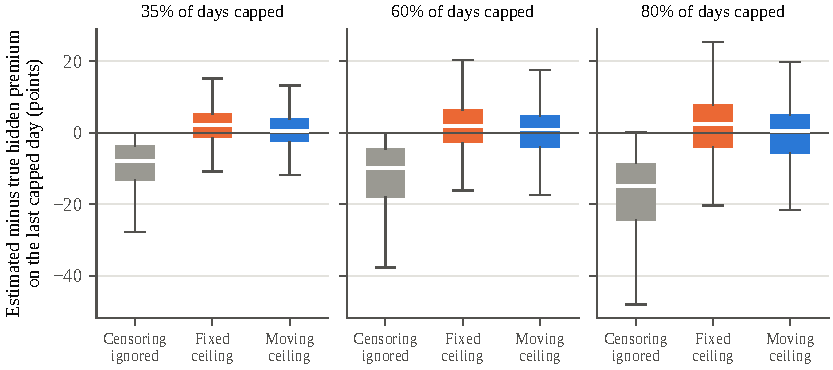
\includegraphics[width=0.95\textwidth]{figures/fig4_montecarlo.pdf}
\caption{Monte Carlo: error in the estimated hidden premium on the last capped day, by estimator and by the share of days capped. Boxes show the interquartile range and the median, whiskers 1.5 times the range. \mcReps{} replications per design; simulated data.}\label{fig:mc}
\end{figure}

\subsection{Supply and float (P3)}
Each dated creation is a supply shock of known size. For every creation event $e$ in fund $i$, the change in the premium from five sessions before to ten sessions after is divided by the percentage change in units, which gives an elasticity $\eta_{i,e}=\Delta\pi_{i,e}/\Delta\ln(\text{units}_{i,e})$. Pooled within a fund, the elasticity implies the increase in units, and so the quota in dollars, that would have closed that fund's premium. The test that creations lower the premium is one-sided and is refuted by a zero or positive mean. Because room is shared within a fund house, outflows from sister schemes are examined as a source of variation in the capacity to create; the premium on each creation date is reported, and market makers are not identified. Across funds the relation between premium and net float is shown as a figure and tested with a rank correlation on the first session of each month after the change. With six funds a regression would add nothing to the picture.

\subsection{Limit-hit dynamics and feeders (S1, S2)}
For the sessions after the change,
\begin{equation}\label{eq:s1}
\Delta\pi_{i,t}=a_i+b_1\,\mathit{TO}_{i,t}+b_2\,d_{i,t}+b_3\,r_{i,t-1}+b_4\,r_{i,t-5:t-1}+b_5\,A_t+\sum_{j=1}^{3}g_j\,H_{i,t-j}+\varepsilon_{i,t},
\end{equation}
with turnover $\mathit{TO}$, delivered share $d$, the fund's own return over the previous one and five sessions, search interest $A$, and indicators $H$ for an upper-limit day $j$ sessions earlier. Resale-option models predict that premium and turnover rise together; extrapolation predicts a positive $b_3$ that survives the inclusion of turnover \citep{pearson2021chinese}; the attention account predicts positive $g_j$ with more and smaller trades. Errors allow for correlation across funds within a day \citep{driscoll1998consistent}. For feeders, the monthly change in ETF units held is set against the lagged premium; with a handful of feeders the evidence is descriptive.

\subsection{What the rule cost buyers}
A policy reader will ask what was paid above the price the old rule would have allowed. For each fund-day after the change,
\begin{equation}\label{eq:excess}
\text{excess rupees}_{i,t}=\text{units traded}_{i,t}\times\max\big(0,\;\overline{P}_{i,t}-1.2\,\NAV_{i,t-2}\big),
\end{equation}
where $\overline{P}_{i,t}$ is the day's average traded price. Summed by fund and week it measures the transfer from buyers to sellers that the old ceiling would have prevented, without any claim about who they were.

\subsection{Inference}
There are at most six treated funds from three fund houses and one rule date. Standard errors clustered by fund are unreliable at this number, as is the wild cluster bootstrap \citep{mackinnon2018wild}. The paper therefore leads with the holiday observation, the rank of the true date among placebo dates and break dates by fund, and uses panel estimates only in support. Tests are few and stated in advance, in the spirit of pre-analysis plans \citep{olken2015promises,harvey2017presidential}.

%=====================================================================
\section{Evidence Available Before the Panel}\label{sec:evidence}
This section reports what can be established now. Tables~\ref{tab:lastday}, \ref{tab:units} and~\ref{tab:cross} are computed from files of the exchange and of the Association of Mutual Funds in India for a few dates, saved by the project as test data for its collectors \citep{nse2026files,amfi2026nav}. Table~\ref{tab:path} mixes those files with press figures and says which is which. None of it tests a hypothesis.

\subsection{The last day of the fence}
The security master dated 4 September 2026 gives each fund's band for 7 September, the first session of the new regime. The band is 10\% either side of the 4 September close, with the lower limit rounded up and the upper rounded down to the paisa, so the close can be recovered exactly. The NAV file gives each fund's NAV for 2 September, and 1.2 times that NAV, rounded down, is the upper limit that applied on 4 September. Table~\ref{tab:lastday} compares the two.

\begin{table}[!t]
\centering\small
\caption{The last session of the NAV-anchored band, 4 September 2026}\label{tab:lastday}
\begin{tabular}{lrrrcrr}
\toprule
 & NAV of & Upper limit, & Close, & Close at & NAV of & Quoted\\
Fund & 2 Sep (Rs) & $1.2\times$NAV (Rs) & 4 Sep (Rs) & the limit & 4 Sep (Rs) & premium (\%)\\
\midrule
\fund{MONQ50} & 118.2753 & 141.93 & 141.93 & yes & 118.7371 & 19.53\\
\fund{MON100} & 270.5591 & 324.67 & 324.67 & yes & 272.9167 & 18.96\\
\fund{MASPTOP50} & 66.5513 & 79.86 & 79.86 & yes & 66.7667 & 19.61\\
\fund{MAFANG} & 172.9741 & 207.56 & 207.56 & yes & 173.6007 & 19.56\\
\fund{MAHKTECH} & 18.4215 & 22.10 & 22.10 & yes & 18.5442 & 19.17\\
\fund{HNGSNGBEES} & 455.4774 & 546.57 & 471.09 & no & 459.4592 & 2.53\\
\addlinespace
\fund{NIFTYBEES} & 272.7284 & 327.27 & 273.27 & no & 272.5784 & 0.25\\
\bottomrule
\end{tabular}
\tabnote{Sources: \citet{amfi2026nav} for NAV; \citet{nse2026files} for the band applying on 7 September, from which the 4 September close is recovered as the only two-decimal price consistent with both limits. For \fund{MONQ50} the recovered close equals the close reported in the press. The quoted premium is the close over the NAV of the same date. \fund{NIFTYBEES} is a domestic ETF shown for comparison.}
\end{table}

Five of the six funds closed at the upper limit to the paisa. NSE's close is the volume-weighted average of the last half hour, or the last trade if there was none, so a close exactly at the limit means that every trade in the closing half hour, or the last trade of the day, was at the limit price. Demand at the ceiling was unsatisfied in five funds on the day the ceiling was removed. The sixth, the Hang Seng fund, closed 2.5\% above NAV; its units have not changed since January 2025 either (Table~\ref{tab:units}), so a block on creation is not sufficient for a premium. Demand is also needed.

The table also shows the moving ceiling of Proposition~\ref{prop:fence} at work. All five funds were at the same limit of 1.2 times a lagged NAV, yet their quoted premiums range from 18.96\% to 19.61\%, because each fund's NAV had moved by a different amount over the two days.

\subsection{The path of one fund}
Table~\ref{tab:path} and Figure~\ref{fig:monq50} trace the Nasdaq Q50 ETF. On 7 September, with US markets shut, the fund's NAV changed by $-0.004\%$, the accrual of expenses, and its price rose 15.6\% \citep{vr2026rs96}: more than the initial 10\% band and the first widening allow, so the band widened twice on the first day. The close reached 235\% above NAV on 18 September, the ninth session. On 21 September the unit traded as high as Rs 471.99, 19.1\% above its base of Rs 396.30 and nearly four times that day's NAV, and closed at Rs 317.04, exactly 20\% below the base. About 4.3 million units changed hands, 29\% of all units outstanding \citep{indmoney2026penny,whalesbook2026}. No news, exchange action or fund-house statement has been reported as a trigger; the fall is treated here as endogenous. A second lower-limit day followed. By 7 October the premium was again above 110\%, and on 9 November the quoted premium was 100.8\%. The six funds together traded about Rs 10,440 crore on the two exchanges in 2026 up to early October, of which a press analysis places Rs 3,094 crore above NAV \citep{businessline2026}.

\begin{table}[!t]
\centering\small
\caption{Motilal Oswal Nasdaq Q50 ETF: close, NAV and quoted premium, 2026}\label{tab:path}
\begin{tabular}{lrrrrl}
\toprule
Date & Session & Close (Rs) & NAV (Rs) & Premium (\%) & Source\\
\midrule
4 Sep & $0$ & 141.93 & 118.74 & 19.5 & Exchange and AMFI files\\
7 Sep & 1 & 164.07 & 118.73 & 38.2 & Close from reported rise; AMFI NAV\\
9 Sep & 3 & 213.01 & 116.42 & 83.0 & Press close; AMFI NAV\\
16 Sep & 7 & 275.28 & 116.69 & 135.9 & Press\\
17 Sep & 8 & 330.25 & 119.15 & 177.2 & Press\\
18 Sep & 9 & 396.30 & 118.14 & 235.5 & Press\\
21 Sep & 10 & 317.04 & 120.23 & 163.7 & Press\\
22 Sep & 11 & 253.64 & 120.17 & 111.1 & Press; value shown is iNAV\\
23 Sep & 12 & 202.92 & 120.59 & 68.3 & Press\\
30 Sep & 17 & 194.62 & 119.68 & 62.6 & Press\\
7 Oct & 21 & 258.57 & 123.09 & 110.1 & Press\\
14 Oct & 26 & 249.83 & 117.96 & 111.8 & Press\\
4 Nov & 40 & 219.38 & 117.76 & 86.3 & Press\\
9 Nov & 43 & 229.67 & 114.38 & 100.8 & Exchange and AMFI files\\
\bottomrule
\end{tabular}
\tabnote{Press sources: \citet{indmoney2026unwind,vr2026rs96,vr2026sep25,vr2026oct2,vr2026oct8,vr2026oct16,vr2026nov6}. Session counts NSE trading days from the change of anchor; 14 September was a market holiday. The close of 7 September is computed from the reported rise of 15.6\%. The premium is the close over the NAV shown. The press reported 81.4\% for 9 September using the NAV of 8 September.}
\end{table}

\begin{figure}[!t]
\centering
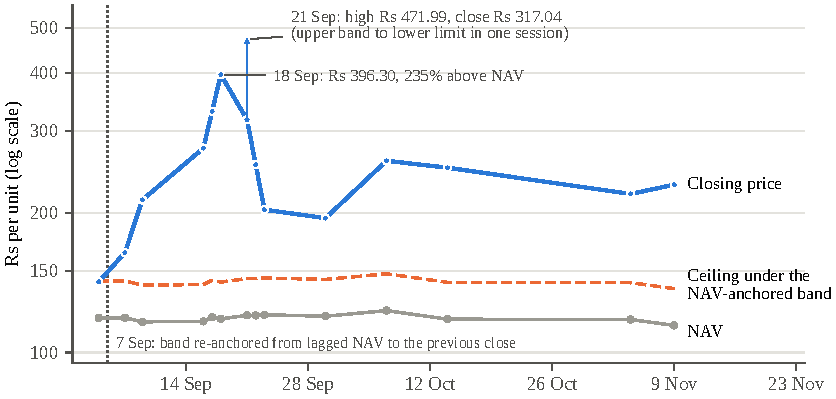
\includegraphics[width=0.95\textwidth]{figures/fig1_monq50.pdf}
\caption{Motilal Oswal Nasdaq Q50 ETF, 4 September to 9 November 2026: closing price, NAV and the ceiling that the NAV-anchored band would have set (1.2 times NAV). Points are the dates in Table~\ref{tab:path}; lines join them. The triangle marks the intraday high of 21 September.}\label{fig:monq50}
\end{figure}

\subsection{Units outstanding}
Table~\ref{tab:units} reports units outstanding from NSE's security master on five dates. Between July 2024 and April 2026 the Nasdaq Q50 ETF's units rose from 3.28 million to 14.68 million, an increase of exactly 19 creation units, in a period that press accounts describe as closed to creation. Eight of the 19 came in the second half of 2024, when the fund's premium was reported between 17\% and 25\%; by May 2025 it had fallen to 1.8\% \citep{vr2025premium}. The Nasdaq 100 ETF added 26 creation units in the second half of 2024 and lost three afterwards. The Hang Seng fund added 179. The two Mirae Asset funds on US indices only shrank. From April to November 2026 no fund's units changed, although one creation unit of the Nasdaq Q50 ETF bought at NAV and sold at the 18 September close would have yielded about Rs 16.7 crore. The fund houses' room was exhausted when it would have been most valuable.

\begin{table}[!t]
\centering\small
\caption{Units outstanding, millions}\label{tab:units}
\setlength{\tabcolsep}{5pt}
\begin{tabular}{lrrrrrr}
\toprule
 & & & & & & Change in\\
Fund & 1 Jul 2024 & 2 Jan 2025 & 1 Apr 2026 & 4 Sep 2026 & 9 Nov 2026 & creation units\\
\midrule
\fund{MONQ50} & 3.275 & 8.075 & 14.675 & 14.675 & 14.675 & $+19$\\
\fund{MON100} & 498.385 & 504.885 & 504.135 & 504.135 & 504.135 & $+26$, $-3$\\
\fund{MASPTOP50} & 172.474 & 168.624 & 168.624 & 168.624 & 168.624 & n.e.\\
\fund{MAFANG} & 253.304 & 248.904 & 247.304 & 247.304 & 247.304 & n.e.\\
\fund{MAHKTECH} & 192.912 & 192.912 & 193.712 & 193.712 & 193.712 & $+1$\\
\fund{HNGSNGBEES} & 19.112 & 23.587 & 23.587 & 23.587 & 23.587 & $+179$\\
\bottomrule
\end{tabular}
\tabnote{Source: \citet{nse2026files}, field \texttt{IssdCptl}; the value for 1 April 2026 is from the project's log of the same file series. Creation-unit sizes as in Table~\ref{tab:funds}; the two Mirae Asset funds on US indices lost 3.85 and 6.00 million units. Reconciliation with fund-house disclosures of assets is pending.}
\end{table}

\subsection{The cross-section on 9 November 2026}
Table~\ref{tab:cross} is a snapshot of all six funds on the most recent date for which files are held. Three things stand out.

\begin{table}[!t]
\centering\small
\caption{The six funds on 9 November 2026}\label{tab:cross}
\setlength{\tabcolsep}{3.9pt}
\begin{tabular}{lrrrrrrrr}
\toprule
 & & \multicolumn{2}{c}{Premium (\%) over} & Value & Value above & Turnover & Delivered & Rupees\\
\cmidrule(lr){3-4}
Fund & Close (Rs) & same-date & last known & at NAV & NAV & (\% of & share & per\\
 & & NAV & NAV & (Rs crore) & (Rs crore) & units) & (\%) & trade\\
\midrule
\fund{MONQ50} & 229.67 & 100.8 & 107.1 & 168 & 169 & 1.87 & 44.5 & 7,514\\
\fund{MASPTOP50} & 96.52 & 50.5 & 53.4 & 1,082 & 546 & 0.35 & 57.8 & 6,770\\
\fund{MAFANG} & 234.91 & 47.2 & 51.4 & 3,945 & 1,864 & 0.39 & 45.9 & 12,251\\
\fund{MAHKTECH} & 21.93 & 34.7 & 33.4 & 315 & 109 & 0.27 & 65.2 & 2,427\\
\fund{MON100} & 298.59 & 16.6 & 20.6 & 12,911 & 2,142 & 0.19 & 52.0 & 12,529\\
\fund{HNGSNGBEES} & 455.52 & 4.3 & 4.2 & 1,030 & 45 & 0.13 & 62.5 & 4,580\\
\addlinespace
Six funds & & & & 19,451 & 4,875 & & & \\
\addlinespace
\fund{NIFTYBEES} & 285.01 & $-0.3$ & $-0.2$ & 73,920 & $-208$ & 0.44 & 54.2 & 43,556\\
\bottomrule
\end{tabular}
\tabnote{Sources: \citet{nse2026files} for prices, traded quantity and value, trades, delivered share and units outstanding (NSE only); \citet{amfi2026nav} for NAV dated 9 November. The last known NAV is the NAV displayed by NSE at the close. Value at NAV is units times the NAV dated 9 November; market value above NAV is units times the close, less value at NAV. \fund{NIFTYBEES} is a domestic ETF shown for comparison.}
\end{table}

First, the sums involved are not small. The six funds held assets worth Rs 19,451 crore at NAV and were priced Rs 4,875 crore above that, a quarter of their value. The largest amounts are in the large funds with moderate premiums, not in the fund with the headline premium: the Nasdaq 100 ETF and the FANG+ ETF account for Rs 4,006 crore of the total. This is what holders stand to lose if premiums close, whether through new room under the cap or through the return of a NAV anchor.

Second, among the four funds on US indices the smallest float carries the largest premium and the largest float the smallest (Figure~\ref{fig:cross}). The Nasdaq Q50 ETF, worth Rs 168 crore at NAV, turned over 1.9\% of its units in a day, ten times the rate of the Nasdaq 100 ETF, and had the lowest delivered share. Small float, high turnover and a large premium together are what models of speculative trading under short-sale constraints predict \citep{hong2006asset}. The figures are gross of feeder holdings and for one day; they motivate P3 and do not test it.

Third, the trades are small. The average trade in the six funds was between Rs 2,400 and Rs 12,500, against Rs 43,600 in the largest domestic ETF. Daily files do not identify investors, but trades of this size are not those of institutions.

\begin{figure}[!t]
\centering
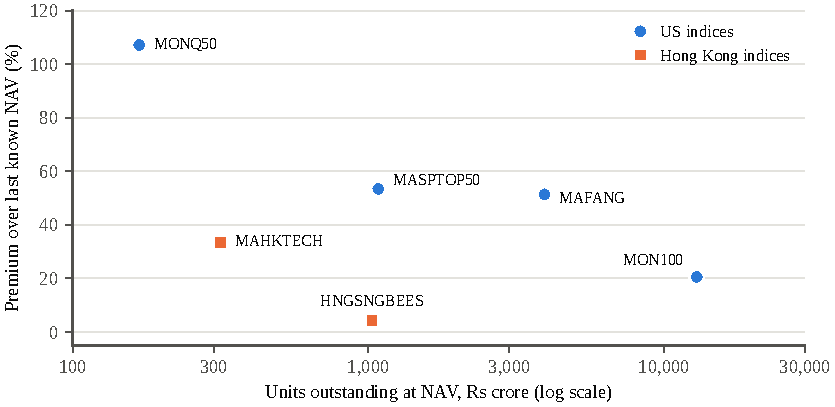
\includegraphics[width=0.92\textwidth]{figures/fig6_cross_section.pdf}
\caption{Premium and float on 9 November 2026. Premium over the last known NAV against units outstanding valued at NAV, gross of feeder holdings (Table~\ref{tab:cross}).}\label{fig:cross}
\end{figure}

\subsection{Reading}
These figures are consistent with P1 and with the supply side of P3, and they contradict the common account that creation has been shut since 2022 or 2024. They do not test either. The premiums between the two file dates are press premiums with the timing defect of Section~\ref{sec:institutions}, units are observed on five dates, and no fair-value series has been computed. What the files do settle is the starting point for P2: on the day the fence came down, five funds were pressed against it.

%=====================================================================
\section{Registered Tests for April 2027}\label{sec:april}
Paragraph 4.4 of the circular makes the previous day's NAV the base from 1 April 2027, subject to exchanges and fund houses resolving operational difficulties. If any NAV anchor is applied, Proposition~\ref{prop:cliff} holds: a fund trading more than 20\% above the anchoring NAV must jump into the band on the first day. A holder who is certain of the switch should not hold through it. The switch is a target, however, and may be delayed, so a premium above the future ceiling is not by itself evidence of irrationality. The tests concern how the excess over that ceiling moves, and they are fixed here before any observation from 2027 exists. The text below will be filed on a public registry before 31 December 2026.

\paragraph{Definitions.} The \emph{excess} of a fund on a day is
\begin{equation}\label{eq:xapril}
x_{i,t}=\ln\!\left(\frac{P_{i,t}}{1.2\times\NAV^{\mathrm{pub}}_{i,t}}\right),
\end{equation}
where $\NAV^{\mathrm{pub}}_{i,t}$ is the last NAV published before that close. An \emph{exposed fund} is one of the six with $x>0$ at the close of the last session of December 2026. The \emph{switch date} $T$ is the first session on which NSE's official band for a fund is centred on a NAV of any lag, read from the security master. An \emph{event} is a dated publication by SEBI, the Reserve Bank of India, NSE, BSE, the Association of Mutual Funds in India or the three fund houses about the band's base, the overseas limits or creation in these funds. Each event is logged with its time and classed, before prices are examined, as premium-reducing (anchor confirmed or advanced, limits raised, creation resumed) or premium-preserving (delay, exemption).

\paragraph{Branches.} A: a NAV anchor is applied to these funds on or before 30 April 2027. B: a delay or exemption is announced before $T$. C: the limits are raised, or an exposed fund's units rise by at least one creation unit, before $T$.

\paragraph{Predictions.} Each prediction names the branch in which it applies.\nopagebreak
\begin{enumerate}
\item \emph{Run, not cliff} (A). For every exposed fund $x\le 0$ at the close of $T-1$. The prediction is refuted for a fund if $x>0$ then, in which case the fall arrives as a jump on $T$.
\item \emph{Path} (A). Between 1 January and $T-1$ each exposed fund has at least one session whose low equals the official lower limit, and its median $x$ over the last 10 sessions before $T$ is below its median over sessions 11 to 40 before $T$.
\item \emph{News} (all branches). Across events and exposed funds, $x$ falls from the close before an event's first tradable session to the close two sessions later for premium-reducing events and rises for premium-preserving ones. An exact sign test is applied to the pooled changes.
\item \emph{Trading} (A, B). Units traded over units outstanding in the 20 sessions before $T$, or before the announcement in branch B, exceed the ratio in sessions 21 to 60 before.
\item \emph{Supply} (C). After units rise, $x$ falls, and by more where the percentage rise in units is larger.
\end{enumerate}
All five predictions will be reported whatever the result.

\paragraph{Known when written.} Press premiums from 4 September to 4 November 2026; exchange and fund-industry files for 4 September and 9 November 2026; units outstanding on five dates; a check of NAV timing for one fund; no price after 9 November 2026; no output of the study's pipeline. This paragraph will be updated on the day of filing.

\paragraph{Why a run is the prediction.} Before $T$ a falling price can lose at most 20\% a day, and on lower-limit days sellers may find no buyers, as on 21 and 22 September 2026. A fund at twice its ceiling needs at least four such sessions to get inside the band (Proposition~\ref{prop:cliff}). Holders who intend to leave must therefore leave early, and each has reason to leave before the others. The alternative is that the premium survives to $T-1$ because holders doubt the date, cannot coordinate \citep{abreu2003bubbles} or do not know the rule. The first prediction separates the two.

%=====================================================================
\section{Threats to Validity and Limitations}\label{sec:limits}
\emph{Few funds.} Six funds from three fund houses cannot support claims about ETFs in general. The contribution is a well-identified case, and inference is chosen accordingly.

\emph{A shared demand shock.} Chinese ETFs on US technology indices also traded at high premiums in September and November 2026 \citep{caixin2026nov}. A global rush into US technology shares could raise premiums in both countries. The China comparison is meant to separate that shock from the Indian rule; it is imperfect because Chinese quotas and subscription limits also changed during the year.

\emph{The latent premium is a model.} The split in~\eqref{eq:split} is relative to a law of motion estimated before the change. If that law would have changed in September 2026 for reasons unrelated to the rule, the change is counted as induced. The covariates, the China comparison and the two-sided form of the test limit the problem and do not remove it.

\emph{Fair value.} Three of the indices have no liquid future of their own, and the exchange rate each fund house uses is not yet documented. Errors of one or two percentage points do not matter at premiums above 50\% but do matter for the censored model near 20\%, which is why results are reported with unit and estimated betas and with the premium over the last known NAV.

\emph{Who buys.} Daily data show delivered share, trade count and trade size, not investor identity. Without account-level data the trading hypotheses distinguish mechanisms only indirectly, and the paper makes no statement about the rationality of any group.

\emph{Short selling.} Eligibility for securities lending is set by rule: an index ETF qualifies if it traded on at least 80\% of days over six months with an impact cost of 1\% or less \citep{bs2012slb}, and the Nasdaq 100 ETF was among the first admitted \citep{bs2013slb}. Three facts remain to be established for 2026: whether the six funds were on the eligible list, whether any units were in fact lent, and whether brokers allowed short sales within the day. Until they are, the paper says only that an overnight short position needed a borrow that we could not observe.

\emph{The rule may change.} SEBI may alter the April target or the limits. The branches in Section~\ref{sec:april} treat each as an event; they do not remove the uncertainty.

\emph{Sources.} Section~\ref{sec:evidence} uses press figures between its two file dates. The date on which the first band regime began has not been established and will be inferred from prices. How fund houses allocate freed room is not public.

\emph{Researcher knowledge.} P1 to P3, S1 and S2 were written after the September and October price path was public. They are predictions only for data not yet assembled. R1 is a prediction in the full sense.

%=====================================================================
\section{Conclusion}\label{sec:conclusion}
India's international ETFs offer an unusual setting: an asset with a published value, a regulatory barrier to arbitrage that can be dated from exchange records, and a price limit whose anchor moved once and is due to move again. The argument of this paper is that the anchor is not a technical detail. Anchored to value, a limit bounds mispricing; anchored to price, it bounds only the speed at which mispricing can grow; and a return from the second to the first forces a jump. Files for the last day of the old rule show five of six funds pressed against the ceiling, and files for 9 November show holders owning units priced Rs 4,875 crore above what the funds hold.

How much of that premium was waiting behind the fence and how much the new rule created is the question the design is built to answer, with an estimator that recovers a known hidden premium in simulation and a test whose size will be calibrated by bootstrap. The next version of the paper will report the estimates. The version after April 2027 will report the outcome of the registered tests, whichever way they fall.

For regulators the case carries a general point. A rule written for assets whose price can outrun a stale value was applied to assets whose price is not tied to value at all, and the property that had kept them near value was a side effect of the rule that was replaced. Where creation can be blocked, a limit on price changes is not a limit on mispricing, and some instrument anchored to value, whether a band, a halt or a call auction, has to do that job.

%=====================================================================
\appendix
\section{Protocol Timeline}\label{app:protocol}
Table~\ref{tab:protocol} lists, for each element of the design, the date it was fixed and what had been seen at that date.

\begin{table}[H]
\centering\small
\caption{Elements of the design and outcomes already seen}\label{tab:protocol}
\begin{tabularx}{\textwidth}{L{3.9cm}L{2.6cm}Y}
\toprule
Element & Date fixed & Outcomes seen at that date\\
\midrule
Fair-value measure \eqref{eq:fv}, \eqref{eq:pi} & 10 Nov 2026 & NAV timing check for one fund; no fair-value series computed\\
P1 to P3, S1, S2; the window of sessions 16 to 40 in \eqref{eq:iota} & 11 Nov 2026 & Press premiums, 4 Sep to 4 Nov 2026; units outstanding on five dates; no output of the study's pipeline\\
Estimator of Section~\ref{sec:design}, its Monte Carlo check and the bootstrap calibration & 12 Nov 2026 & As above, plus exchange and fund-industry files for 4 Sep and 9 Nov 2026 (Tables~\ref{tab:lastday} and~\ref{tab:cross}); simulated data only\\
R1 and the tests of Section~\ref{sec:april} & 11 Nov 2026 (text); registration pending & As above; no price after 9 Nov 2026\\
\bottomrule
\end{tabularx}
\end{table}

\section{Monte Carlo Design}\label{app:mc}
\emph{Data-generating process.} The latent log premium follows $\pi^{*}_{t}=\mu(1-\rho)+\rho\pi^{*}_{t-1}+\sigma\varepsilon_t$ with $\rho=0.985$, $\sigma=0.02$ and $\mu\in\{0.10,0.20,0.30\}$, started from its stationary distribution. Daily log changes in value are $n_t\sim N(0,0.012^2)$ and the ceiling is $c_t=\ln 1.2-(n_t+n_{t-1})$. For $t\le 400$ the observed premium is $\min(\pi^{*}_t,c_t)$. A replication is kept if the last pre-change day is capped and between 10\% and 95\% of pre-change days are capped. For $t>400$ the observed premium is $\pi^{*}_t+\delta$ with $\delta\in\{0,0.3,0.6\}$.

\emph{Estimators.} (i) Ordinary least squares of the observed premium on its lag. (ii) Maximum likelihood for~\eqref{eq:latent}--\eqref{eq:obs} applied to the premium over the band's base, $\pi_t+(n_t+n_{t-1})$, with the fixed ceiling $\ln 1.2$. (iii) Maximum likelihood for~\eqref{eq:latent}--\eqref{eq:obs} with the moving ceiling $c_t$. For (ii) and (iii) the likelihood is computed by the recursion~\eqref{eq:filter} on a grid of 193 points from 0.02 to 1.30 and maximised by the Nelder--Mead method from the least-squares estimates.

\emph{Outcomes.} The hidden premium on day 400 is the mean of the filtered density, compared in levels with the true latent premium. The forecast is 1,500 paths simulated from the filtered density; the 5th and 95th percentiles of the average log premium over sessions 16 to 40 form the band. The plug-in band holds the parameters at their estimates. The band with parameter uncertainty draws one parameter vector per path from a normal distribution centred on the estimates, with the inverse numerical Hessian of the log-likelihood as covariance (for the first estimator, the least-squares covariance). The induced share is~\eqref{eq:iota}. The true induced share is computed from the simulated latent path. The code, \texttt{mc\_censored.py}, is in the \texttt{analysis} folder beside the source of this paper; seeds are fixed, and a replication takes about four seconds.

\section{Variable Definitions}\label{app:variables}
\begin{table}[H]
\centering\small
\caption{Variables in the fund-day panel}\label{tab:variables}
\begin{tabularx}{\textwidth}{L{3.2cm}YL{3.4cm}}
\toprule
Variable & Definition & Source\\
\midrule
Close, last, high, low, average price & NSE daily prices; the close is the average of the last half hour & NSE bhavcopy\\
Same-date NAV & NAV dated $t$ & AMFI\\
Last known NAV & Last NAV whose underlying market had closed before 15:30 on $t$, with its date & AMFI, calendars\\
Fair value $\FV$ & Last known NAV moved to 15:30 by the index future and the rupee rate, eq.~\eqref{eq:fv}, with $\beta=1$ and with estimated $\beta$ & Terminal export\\
Premium $\pi$ & $\ln(\text{close}/\FV)$; main dependent variable & Derived\\
Quoted premium & Close over same-date NAV, less one; for comparison with the press only & Derived\\
Band low, band high & Official band for session $t$ & NSE security master of the previous session\\
Ceiling $c$ & $\ln(\text{band high}/\FV)$, eq.~\eqref{eq:cap} & Derived\\
Limit indicators & High at the initial upper limit; at the maximum limit; last trade at the limit; and the same for the lower limit & Derived\\
Regime & Base that reproduces the band's midpoint: NAV of $t-2$, previous close, NAV of $t-1$ & Derived\\
Units & Units outstanding: daily from July 2024; monthly assets over NAV before & NSE security master; fund houses\\
Creation event & Signed change in units over the creation-unit size & Derived\\
Rationed & One when $\pi>0.02$ and no creation in the previous 20 sessions & Derived\\
Feeder units & ETF units held by feeder funds, monthly, carried forward & Monthly portfolios\\
Net float & (Units less feeder units) times last known NAV & Derived\\
Turnover & Units traded on NSE and BSE over units outstanding & NSE, BSE\\
Delivered share, trades, trade size & Share of traded quantity delivered; number of trades; value per trade & NSE bhavcopy\\
Own returns & Log price return over the previous one and five sessions & Derived\\
Attention & Google Trends daily index for fixed terms, chained across windows & Google Trends\\
Excess $x$ & $\ln(\text{close}/(1.2\times\text{last published NAV}))$, eq.~\eqref{eq:xapril} & Derived\\
Excess rupees & Units traded times $\max(0,\text{average price}-1.2\times\NAV_{t-2})$, eq.~\eqref{eq:excess} & Derived\\
\bottomrule
\end{tabularx}
\end{table}

\section{Chronology}\label{app:chronology}
\begin{table}[H]
\centering\small
\caption{Dated events}\label{tab:chronology}
\begin{tabularx}{\textwidth}{L{2.6cm}YL{3.3cm}}
\toprule
Date & Event & Source\\
\midrule
Apr 2008 & Industry limit on overseas investment by mutual funds set at US\$7 billion & \citet{lawasia2026}\\
5 Nov 2020 & Limit per fund house raised to US\$600 million & \citet{bs2020limit}\\
3 Jun 2021 & Limit per fund house raised to US\$1 billion; US\$300 million per house within US\$1 billion for foreign-listed ETFs & \citet{bs2021limit}\\
18 Jan 2022 & Motilal Oswal suspends issuance of units in its two Nasdaq ETFs & \citet{bs2022motilal}\\
1 Feb 2022 & Fresh overseas subscriptions stop across the industry & \citet{pti2022resume}\\
Jun 2022 & Funds may resume up to each house's room as of 1 February 2022 & \citet{pti2022resume}\\
8 Feb 2023 & Reserve Bank of India: no proposal to raise the limit & \citet{bs2023rbi}\\
5 Jan 2024 & Mirae Asset stops direct creation in its three overseas ETFs & \citet{mirae2024addendum}\\
1 Apr 2024 & Pool for foreign-listed ETFs full & \citet{zerodha2024etf}\\
5 Jan 2025 & Motilal Oswal pauses existing instalment plans in its Nasdaq 100 feeder & \citet{et2025motilal}\\
Oct 2025 & Silver ETFs trade about 10\% above indicative value in a shortage of metal; fund houses suspend feeder subscriptions & \citet{bs2025silver}\\
Late Jan 2026 & Gold and silver outrun the NAV-anchored band; interim base for bullion ETFs & \citet{sebi2026cp}\\
13 Feb 2026 & SEBI consultation paper on base price and bands & \citet{sebi2026cp}\\
15 Jun 2026 & SEBI circular: base is the previous close; NAV base targeted for 1 April 2027 & \citet{sebi2026circular}\\
28 Aug 2026 & Start moved from 1 to 7 September & \citet{sebi2026ext}\\
1 Sep 2026 & NSE implementing circular & \citet{nse2026circular}\\
4 Sep 2026 & Last session of the NAV-anchored band; five of six funds close at the upper limit & Table~\ref{tab:lastday}\\
7 Sep 2026 & Previous-close anchor in force; US markets closed & \citet{nse2026files}\\
18 Sep 2026 & Nasdaq Q50 ETF closes 235\% above NAV & \citet{indmoney2026unwind}\\
21--22 Sep 2026 & Nasdaq Q50 ETF: two lower-limit closes & \citet{indmoney2026unwind}\\
25 Sep 2026 & NSE and BSE press releases cautioning investors & \citet{nse2026press,bse2026press}\\
7 Oct 2026 & NSE repeats its caution & \citet{reuters2026nse}\\
9 Nov 2026 & Six funds priced Rs 4,875 crore above NAV & Table~\ref{tab:cross}\\
1 Apr 2027 & Target date for a base of the previous day's NAV & \citet{sebi2026circular}, para.\ 4.4\\
\bottomrule
\end{tabularx}
\end{table}


\bibliographystyle{plainnat}
\bibliography{refs}
\end{document}
